\documentclass[letterpaper,12pt,oneside]{book}
\usepackage[top=1in, left=1in, right=1in, bottom=1in]{geometry}
%-----------------------__--------
%https://es.overleaf.com/project/642e50d937469ff17340bdc4
% Tesis UNAM https://tex.stackexchange.com/questions/234265/unam-thesis-title-page-portada-tesis-unam

%\usepackage{parskip} % Add the parskip package

\usepackage{setspace} % Add the setspace package
\setstretch{1.5} % Set line spacing to double

\usepackage{pdfpages}
\usepackage{lipsum}

\usepackage[T1]{fontenc}
\usepackage[utf8]{inputenc}
\usepackage[spanish,es-nodecimaldot,es-tabla]{babel}
\usepackage{graphicx}
\usepackage{tikz}
\usepackage{setspace}


%Subfiguras
\usepackage{caption}
\usepackage{subcaption}

% Para referencias 
\usepackage{hyperref}
\usepackage{apacite}
\usepackage{url}

%\addbibresource{CARDIAC}


\title{E-CARDIAC: La evolución hacia un modelo concurrente y paralelo}

\begin{document}
	\frontmatter
	\pagestyle{plain} % Set page style to "plain" for the front matter
	%\maketitle

    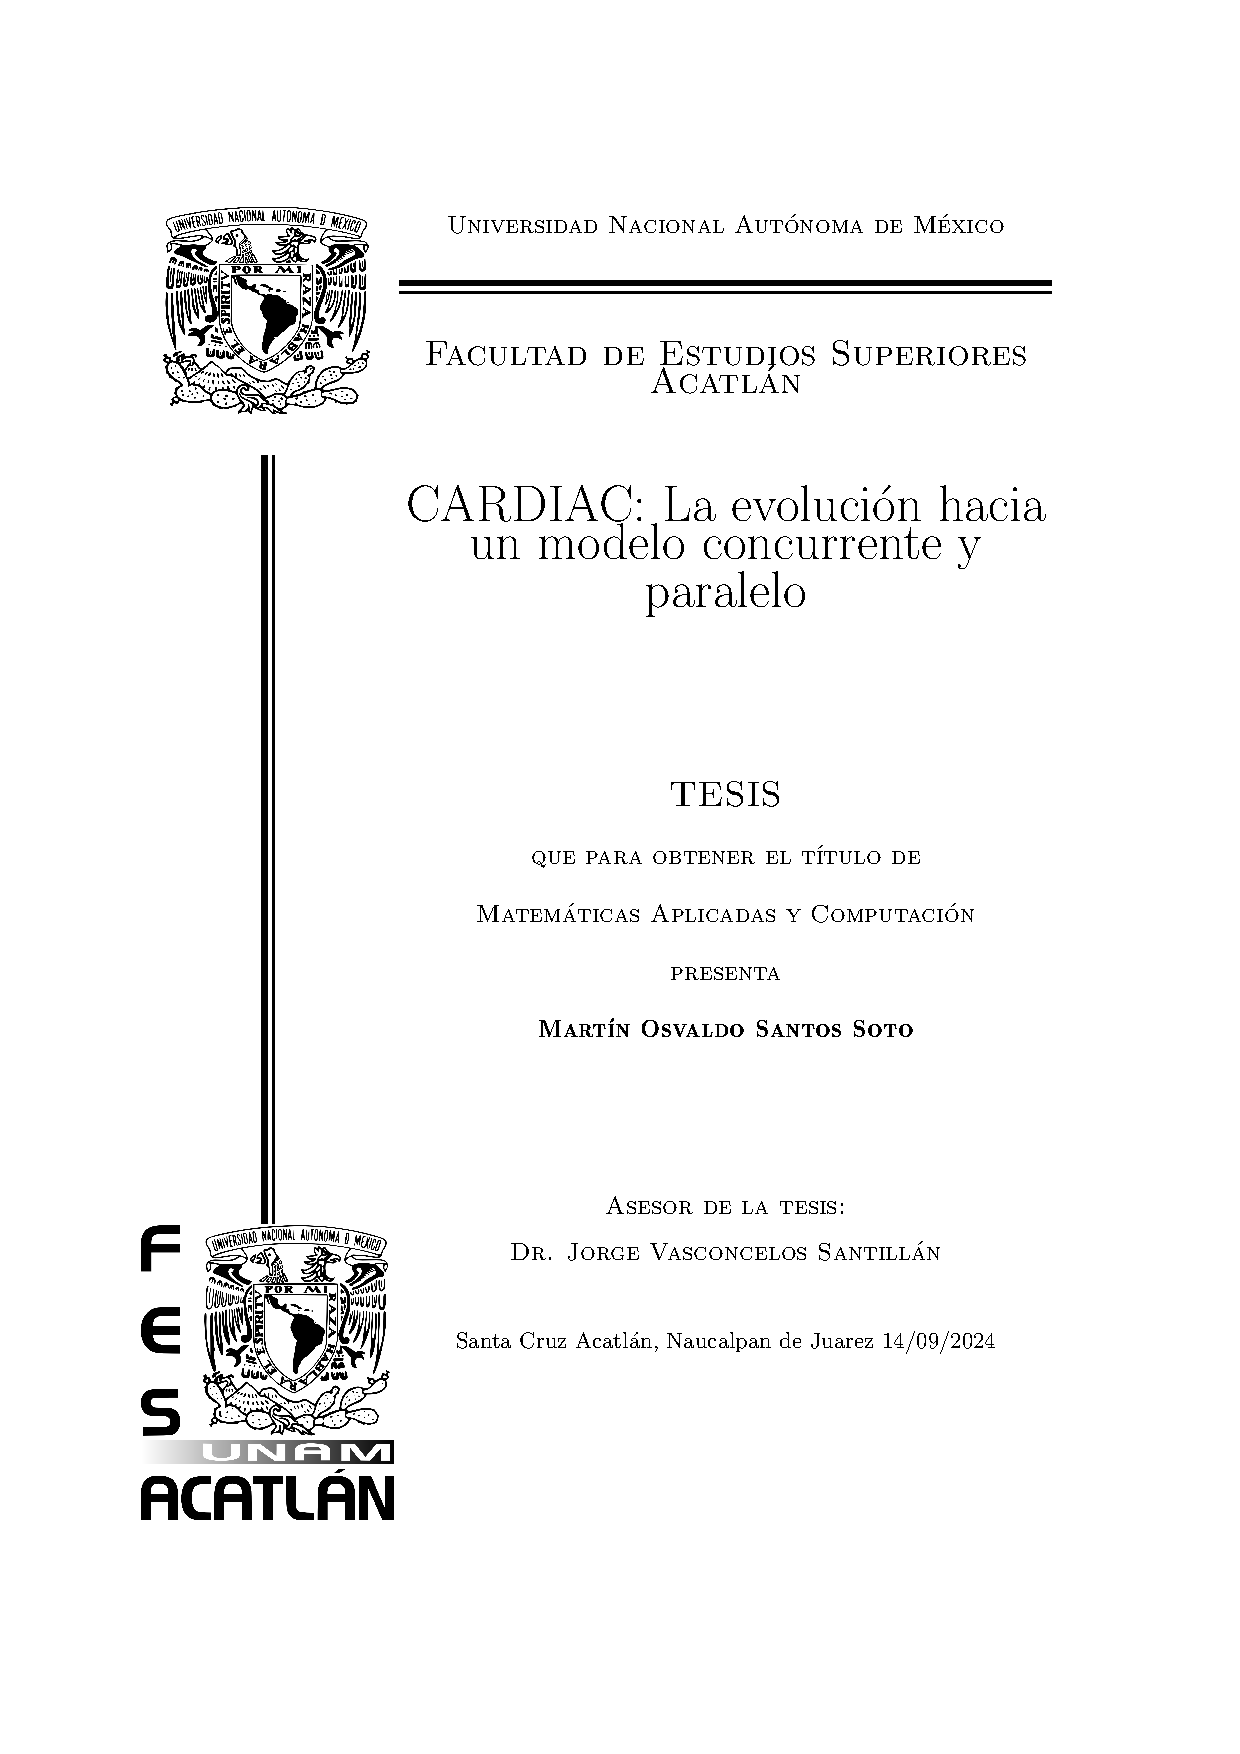
\includepdf{media/cover.pdf}

%---------------------------------
\chapter*{}
\begin{flushright}%
  \emph{``These are fast-moving times, and those who make no effort to understand computers may very well get left behind''}
  
  
  - David W. Hagelbarger, 1968
  %%\thispagestyle{empty}
\end{flushright}

\chapter*{Agradecimientos}
%\spacing{1.5}%\doublespacing

\chapter*{Abstract}

\chapter{Introducción}

	Hoy en día tenemos multitud de aparatos electrónicos que pueden ser llamados computadoras; celulares, laptops, tabletas, relojes inteligentes, y un sin fin más. 
	Estos aparatos pueden ser llamados así siempre que sean  capaces de resolver operaciones aritméticas y lógicas, guardar datos  y procesarlos, y recibir instrucciones del 
	usuario, al menos en la definición
	más aceptada que recoge el diccionario de Oxford (dado que la palabra de origen es anglosajona en este contexto),
	por que sin analizamos más detalladamente el termino ``computadora''  notaremos que el origen de la palabra es anterior a las computadoras
	tal cual las conocemos hoy día, por ejemplo las primeras nociones de ``computadoras''  eran referidas a mujeres de los años 1930 en estados unidos
	que trabajaban en la NASA y realizaban cálculos manuales(la otra definición aceptada en el diccionario es ``persona que hace cálculos manuales''), por ende podemos afirmar que ese termino fue cambiando hasta ser lo que es hoy.
	Si analizamos la historia notaremos que el avance científico en cuanto a maquinas
	que pudieran automatizar tareas que realizaba la humanidad estaban centrados en las calculadoras, había que hacer los cálculos matemáticos menos
	complejos, ya sea con técnicas como los logaritmos y las tablas de multiplicar que se tenían
	para consultar más rápidamente operaciones complejas y repetitivas o con la invención de maquinas que pudieran automatizar calculos, pero con el tiempo el mismo desarrollo de estas maquinas dio paso a algo más,
	a una maquina de propósito general, programable y que ya no solo resolvía operaciones aritméticas, sino que hacía pruebas lógicas y podías
	adaptarla a problemas más particulares, así se fueron formando las ``computadoras'', que como podemos notar son un tipo de evolución de las calculadoras en el sentido de los usos y objetivos
	que tenían al principio. Por ende parece coherente que	de las mujeres que trabajaban haciendo cálculos en la NASA manualmente se les llamase ``computadoras'' por que hacían cálculos manuales
	de forma repetida y que de ahí tomarán el nombre los aparatos más sofisticados que se empezaron a ver en la década de 1940 que resolvían estos problemas y que ahora conocemos con el nombre de ``computadoras''.
	%Sinonimos?
	%%https://www.smithsonianmag.com/science-nature/history-human-computers-180972202/
	
	Para ahondar en está relación de las calculadoras y las computadoras hay que regresar al siglo 19, e ir un poco a los orígenes de la computación,
    más precisamente en el año 1830, con el entusiasta Charles Babbage, que había desarrollado una maquina llamada ``Differential Engine''
	que resolvía ecuaciones matemáticas, una calculadora potente si lo queremos ver desde otra perspectiva. Pero su empeño en los siguientes años 
	se centraría en el diseño y constricción
	de su ``Analytical Engine'', que aunque fue imposible de construir por la tecnología de la época, ya fue pensada como una computadora
	de propósito general, en el sentido que podía hacer cálculos y resolver operaciones lógicas además de que era una maquina que se podía programar,
	cumpliendo así todos los puntos básicos para poder ser considerada como una computadora, lamentablemente no pudo llegar a ver la luz de la mano
	de su creador por las limitantes técnicas de la época, pero dejo un precedente.
	
	En esté sentido podemos ver que las computadoras, o más bien su creación ha llevado mucho tiempo para concretarse en lo que tenemos hoy, que es algo mucho
	más complejo que una calculadora, y aunque sabemos de la complejidad de estos aparatos cuando vemos alguno ¿analizamos como es que funcionan por dentro? ¿como podemos enviar mensajes de texto mientras escuchamos una canción? ¿hay algún programa que ejecuta a los programas que utilizamos? ¿hay un programa que da inicio a todos los procesos de una computadora?
	usualmente la respuesta es ``No'', que no es necesariamente una respuesta mala, en el día a día no podemos detenernos a analizar cada artefacto que tengamos cerca o usemos, a pesar de que sería muy útil saberlo,
	si funciona el aparato es todo lo que necesitamos saber, después de todo hay muchos artefactos o situaciones
	a las cuales prestar atención. Sin embargo, para los profesionales del área de la computación o tecnología en general, así como a aquellos interesados
	por estás tecnologías son preguntas que no pueden faltar. Y es que incluso si tu trabajo es el desarrollo web o
	el diseño de gráficas(que parecieran disciplinas muy lejanas al funcionamiento de un ordenador) entender las razones por las cuales tu computadora o las computadoras para las cuales desarrollas programas pueden hacer cómputos
	en paralelo o tener la potencia que tienen es fundamental para poder optimizar tus desarrollos en la web, los videojuegos que se crean o las gráficas tan detalladas que tenemos en muchos archivos de multimedia; que decir si tu trabajo es la parte del hardware, en ese
	caso debes estar totalmente involucrado con el funcionamiento interno de las computadoras.
	Más aún, considero que al igual que en toda disciplina la historia de la misma o de los artefactos que estudia está debe ser conocida por
	los interesados en la disciplina, pero sobretodo por los profesionales, dado que hay que entender como ha sido la evolución, lo que ha cambiado,
	aquello que a pesar de los años sigue vigente y la razón por la cuál sigue vigente.
	
	
	Centrándonos en el último punto, la historia, es uno de los apartados que a muchas personas les puede parecer tedioso o complicado, 
	por que a pesar de que la historia de las computadoras modernas es corta hablando del tiempo
	de la humanidad, es larga a nivel de la evolución que ha habido en los últimos 80 años, y esto es lo que puede parecer realmente tedioso, sólo hay que ver las diferencias entre
	las computadoras actuales y aquellas que corrían con Windows 98, la diferencia ya es enorme. Ahora si vamos más  a las primeras computadoras personales
	que aún corrían unicamente con línea de comandos y con un paradigma de uso muy diferente al nuestro podemos notar que el cambio ha sido gigante, con todos estos
	cambios uno podría llegar a pensar que una computadora actual ya no tiene prácticamente nada que ver con los ``gigantes de hierro'' de los años 1950, 
	al menos superficialmente se encuentran lejos, pero, internamente de hecho hay muchas similitudes entre estás computadoras. Es más a día de hoy la arquitectura, la estructura
	más general de una computadora actual es exactamente la misma que la de varias de las primeras computadoras, con mejoras en la potencia de
	procesamiento lógicamente, pero con una misma estructura y entender por que esa estructura se ha mantenido vigente hasta nuestros días nos
	llevará a entender lo importante y disruptiva que fue su creación, además de la razón del por que no ha cambiado en todo esté tiempo. Analizando la historia de esa manera, estableciendo conexiones y conociendo que fue lo que continuo
	y aquello que no, ayuda a que esa gigantesca línea del tiempo de las computadoras adquiera otro tono, un tanto menos lleno de datos, que no se quede
	sólo en un montón de fechas y que más bien sea una guía de cambios o sucesos que moldearon el mundo de la computación a lo que hoy conocemos. De está forma podemos conectar los dos puntos que comentaba en el párrafo anterior,
	comprender el funcionamiento de una computadora y conocer la historia de su creación.
	
	 
	Estás preguntas, este análisis principalmente sobre el funcionamiento de las computadoras se dio a lo largo de mi carrera universitaria, y en ese tiempo me di cuenta de lo complejo que podía ser entender
	como funcionaban, después de todo tenía, en principio, la barrera del idioma, dado
	que la lengua franca de la computación es en inglés muchos escritos están en ese idioma, y aunque hay variedad de textos traducidos, otros más,  los más especializados
	o más antiguos es difícil tenerlos en español. Otro tema adicional está en los libros más técnicos, estos 
	manuales
	o libros llenos de teoría acerca del funcionamiento de los ordenadores, la concurrencia, los ordenadores en distribuido, de como funciona el paralelismo, de las necesidades y utilidad del sistema operativo, presentan otro problema además
	del idioma, 
	son realmente difíciles de leer para un estudiante que va empezando en la carrera. Lo curioso es que este problema no es nuevo, ya se habían enfrentado a el no solo muchos
	estudiantes desde la aparición de la computación, sino también muchas instituciones y empresas que querían que más personas aprendieran a usar una computadora,
	aunque cabe aclarar que éste problema cuando empezó a aparecer era un poco distinto por no decir bastante más complejo, y es que esto sucede en los años 60 y 70, cuando se empiezan a popularizar las computadoras, si querías usar una computadora tenías que entender muy bien el como funcionaba por que 
	no había una interfaz gráfica o un sistema operativo que hiciera todas las tareas secundarías por ti, tenías que entender como se movía por dentro la computadora para
	poder programar y resolver tus problemas, además de que tu acceso era muy limitado por lo que no podías perder el tiempo. Es aquí, en este periodo histórico, más precisamente en los años 60, cuando varias compañías e instituciones
	educativas comienzan a lanzar ciertos modelos, manuales y kits para que los estudiantes aprendieran a usar las computadoras
	, algunos básicamente eran un kit de papel con un manual, una ``computadora de papel'' como se les ha llamado, en la cual tu como estudiante
	podías ver como eran las ejecuciones del código que habías escrito, y como eso se materializaba en una respuesta a tu problema inicial. Una de estás fue 
	``Little Man Computer(LMC)'' creada por Stuart Madnick y Jhon Donovan del MIT en los años 60, que con un reducido set de instrucciones permitía a los estudiantes probar la
	ejecución de programas como si estuvieran en una computadora real, otra de mucha relevancia fue su contemporánea CARDIAC(CARDboard Illustrative Aid to Computation) 
	desarrollada por Bell Labs de la mano de David W. Hagelbarger y Saul Fingerman, que es
	muy similar a lo descrito sobre LMC, pero con su propio lenguaje y su propia arquitectura, que incluso llego a ser  más popular
	por el poder de Bell Labs en aquellos tiempos que logro distribuirla en muchas instituciones educativas de estados unidos.
	Lo cual no fue realmente difícil por que en  los años de 1960 
	las computadoras eran ordenadores gigantes y conseguir tiempo para usarlos era realmente difícil, comprarlos directamente imposible para las personas
	comunes, entonces la solución que encontraron para que los estudiantes pudieran practicar fue la creación de estos kits con computadoras de papel, que los
	preparaban  para cuando pudieran usar una computadora ``real''.
	 Hubo otros desarrollos en años siguientes que tuvieron el mismo fin, dado que lo común en los años posteriores y quizá hasta hace algunos años en algunas partes del mundo, fue que acceder a las computadoras reales era o es casi imposible,
	además de que hay más razones por las cuales estos modelos nos pueden ser realmente útiles.

%%link al kit armable
	Eso quizá nos pueda parecer una simple clase de historia de la computación, pero no lo es, CARDIAC sigue siendo muy útil, por que como mencioné, hay más razones por las cuales nos sigue siendo ayudando, de hecho
	funciona para explicar una buena parte del funcionamiento de a las computadoras de una forma sencilla pero a la vez precisa, yo experimente el uso de CARDIAC en una clase de programación paralela y concurrente en la 
	cual esté modelo
	fue fundamental para entender los conceptos básicos de los que parte la computación. También hay que ser consientes que con un modelo cómo CARDIAC no te vas a volver un experto en 
	el funcionamiento de las computadoras,
	pero el punto es entender de una forma clara su estructura de modo que tengas las bases para entonces ser capaz de leer uno de esos manuales llenos de teoría sobre sistemas
	operativos y arquitectura de computadoras con muchísimos conceptos técnicos, los cuales si no tienes cierto conocimiento de base terminan siendo muy complicados de leer y entender.
	
	Aún con todas estás ventajas de CARDIAC, las limitaciones son evidentes, fue construida en el año 1968, no es apta para la concurrencia ni el paralelismo, o 
	incluso un computo distribuido, por esa razón muchas personas que están en el mundo de la computación en los años posteriores han seguido haciendo
	modelos similares como MARIE(Machine Architecture that is Really Intuitive and Easy) o directamente evoluciones de ella como TIMBA(Terrible Imbecile Machine for Boring 
	Algorithms), algunos más técnicos que otros, y aunque la mayoría están en inglés hay varios proyectos en español. 
	Al adentrarme más en estos modelos me di cuenta que un buen modelo que explicará el funcionamiento de computadoras más recientes en los componentes de su arquitectura se volvían más técnicos, como el 
	desarrollo mexicano de \textit{8 bit a complete Design}, 
	que es un gran trabajo, pero que termina usando bastantes conceptos que requieren ciertas bases de conocimiento y aquellos que no son tan técnicos caen un poco en ser bastante similares a CARDIAC, lo cual no 
	es malo, e incluso tiene muchas ventajas que mejoran algunas lagunas de CARDIAC, pero hay otras más que no intentan solucionar por diversas razones. Es en esté punto en el que decidí empezar este
	proyecto de investigación para explicar como funcionan las computadoras de una forma simple y didáctica para aquellos estudiantes que van empezando la carrera
	como forma de contestar esas preguntas tan generales que plantee al principio,
	tomando como base el  desarrollo de CARDIAC y llevándola unos pasos más allá en nivel de arquitectura para que sea capaz de explicar
	la computación concurrente y paralela, así como entender la necesidad de un sistema operativo en maquinas más complejas sin dejar de lado la simplicidad que la 
	caracteriza.
	Con un enfoque particular que lleve al lector a ver las necesidades de hardware y software que hacen evolucionar a CARDIAC,
	de forma que se entienda la razón de la evolución de las computadoras en varios ámbitos fundamentales, y en ese mismo sentido situarse en la línea
	temporal en que surgieron esos cambios para entender su contexto histórico y como lo mencione antes, entender por que hay características  que siguen vigentes
	80 años después en los ordenadores y otras 	que no.
	
	
	Más allá del recorrido en la construcción y diseño de modelos ``evolucionados'' de CARDIAC para computación paralela y concurrente el texto se verá acompañado,
	tal como la clásica CARDIAC distribuida por Bell Labs, con un ``kit'' que incluye un programa que contendrá tres maquinas virtuales, uno para cada
	modelo de CARDIAC, con la diferencia de que estas maquinas virtuales ya no serán en papel, sino interfaces gráficas para uso en computadoras de escritorio con la idea de que sea fácil para el estudiante
	entender la teoría y practicarla, poder ver como se van ejecutando los programás que ya en una versión paralela o concurrente sería un poco más difícil de ver con una computadora de papel dada la cantidad de información que se tiene que almacenar.
	
	%%Le falta algo al cierre%%



\tableofcontents
\listoffigures

\mainmatter

\chapter{Historia de la computación} %


	\section{Breve recorrido por el pasado}
		\subsection{Antecedentes}
		% Maquinas parecidas a las computadoras, que no lo son
		
		Desde que los humanos empezamos a hacer cálculos en el sentido de sumar o restar cantidades representadas por números	hemos necesitado de herramientas
		que nos apoyen en la resolución del calculo, y entre más complejo el calculo necesitamos herramientas más complejas. Es curioso pensar que las
		primeras herramientas para apoyarnos en estos cálculos fueran los dedos de las manos en la lejana Sumeria del milenio 4 a.c. cuando empezaban
		los cálculos de una ``naciente'' contabilidad, que después evolucionaría a lo que hoy conocemos popularmente como \textbf{ábaco}, discutida-mente
		creado por los chinos o babilonios alrededor del año 1010 A.C, y que tras muchos sucesos llegaríamos a tener hoy en día una maquina que no sólo
		resuelve operaciones aritméticas, sino que resuelve casi cualquier problema que pueda ser descrito por instrucciones que se puedan transcribir
		al ``lenguaje'' que entiende la maquina y que a su vez estás instrucciones tengan un resultado, así es, me refiero a la \textbf{computadora}. Pero
		para pasar del ábaco a la computadora tuvieron que pasar muchas cosas, aunque podemos afirmar con total seguridad que el ábaco si bien no cumple
		las cualidades de una computadora como algunos piensan, se puede definir como un \textit{antecesor} de las computadoras.
		% Fuentes de babilonios, cualquier problema que pueda ser descrito?
		
		%% Ser más claro para la definición de lo que ingresa a la computadora
		
		Vamos a trazar está relación llenando los huecos que he dejado en medio, continuando con el siguiente avance de relevancia en cuestión de 
		resolución de operaciones aritméticas, las \textit{calculadoras mecánicas}. Para el año 1600 en plena era del renacimiento en Europa las
		operaciones aritméticas se habían vuelto más complejas, un ejemplo claro eran los cálculos que los navegantes tenían que hacer, o
		los cálculos en astronomía, que llegaban a involucrar muchas multiplicaciones, lo que los volvía muy complejos. Por esas
		necesidades en 1614 el matemático escoses Jhon Napier publico su descubrimiento sobre logaritmos, los cuales permiten
		convertir las multiplicaciones en sumas gracias a sus propiedades, pero si bien estos aminoraban el problema, no
		lo solucionaban del todo, de hecho había muchas tablas de logaritmos ya calculados de muchos números para hacer los
		cálculos más rápido, es por ello que empiezan a surgir dispositivos mecánicos que podían realizar estos cálculos y otros
		de manera más veloz, dos ejemplos de esto son ``The Gunter Scale'' creada por Edmund Gunter y ``The Slide Rule'', que de hecho
		está última sigue usándose en las áreas de ingeniería para calcular logaritmos o ciertas funciones aritméticas. Un poco
		más lejos llegarían Pascal y Leibniz con sus inventos, que ya serían calculadoras en forma, Leibniz inventaría la
		``Step Reackoner'' que permitía hacer cálculos aritméticos en el año de 1973, basada en ``The Pascaline'' o ``Arithmetic Machine'' creada
		por Pascal en 1964; Ambas ya podían ser llamadas calculadoras funcionales, aunque ya desde muchos años antes se venía pensando
		en un dispositivo como la calculadora, de hecho Leonardo Da Vinci  dejaría sus planos para construir una(la cual no pudo construir) que
		ingenieros de la época moderna pudieron seguir para crearla. Podemos notar que las inquietudes por automatizar operaciones estaban
		ya desde antes que la tecnología de su época les permitiera a los inventores llevar a cabo sus planes, pero que a pesar de esto las siguientes
		generaciones siguieron adelante con esas ideas, a veces independientemente y otras usando de base lo que ya existía de antes, para
		continuar con la innovación; este interesante patrón lo veremos de nuevo más adelante.
		%Slide rule en ingenieria
		
		Aunque las maquinas de Leibniz y Pascal eran calculadoras en forma, su replicación no era tan fácil y tampoco fueron muy populares, pero
		si hay una época dónde replicar maquinas para automatizar procesos va a estar en su auge esa es la \textbf{revolución industrial}. En
		1820 un francés llamado Charles Xavier Thomas de Colmar construyo el ``Arithmometer'', basándose en la terminología de Leibniz, fue la primer
		calculadora en forma que se vendió masivamente, aunque era gigante, era revolucionaría para la época y resolvía muchos problemas, tal fue
		su éxito que se vendió por 90 años.
		
		El antecesor directo de la computadora, y sucesor cuasi directo del ábaco no sólo había nacido, sino que ya había conseguido llegar a gran parte de
		la población, así que, si ya se había logrado el reto, ¿cuál era el siguiente? ¿hacerla más pequeña? si, más pequeña para que pudiera llegar a más personas,
		más veloz y que pudiera hacerse más fácil el uso para el usuario, al menos esa sería la respuesta general, ¿cual sería la de un visionario? Alguien
		que piensa más allá de las convenciones quizá pensaría un dispositivo que fuera capaz de resolver más que solo problemas aritmeticos. Y ese era Charles Babbage,
		un reconocido matemático de su época, miembro fundador de la ``Royal Astronomical Society'' en 1920, inventor, pionero en la investigación
		de operaciones, alguien muy distinguido en su época sin duda. Para el año de 1922 estaba diseñando su ``Diferential Engine'', una maquina totalmente mecánica que iría más allá de las
		calculadoras convencionales, resolvería funciones polinómicas e incluso tendría almacenamiento, pero que no llegaría a ser producida, en parte
		por lo difícil que era en la época, y en parte por que Charles ya estaba pensando en algo incluso más grande, para el año 1833 el mecanicista
		que había sido contratado para construir la maquina renuncio y la maquina quedo inconclusa.
		
		Lo que Charles ya estaba pensando, y de hecho en 1933, cuando se dio por terminada la construcción de la maquina diferencial, ya estaba decidido a construir era la 
		``Analytical Engine'', una maquina de computo más general que la anterior y que resolvía más operaciones. A diferencia de las calculadoras del momento, está maquina 
		tendría cuatro secciones principales, 
		el almacenamiento, un impresor, es decir que imprimiría en
		tablillas los resultados para que fuese más automática, un molino(``the mill'') que sería análogo al CPU que hoy conocemos pues ahí
		se llevarían a cabo las operaciones y un lector de instrucciones; las cuales la diferencian de las calculadoras de esa época solo tenían un resolutor de
		operaciones similar al ``molino'' y a lo mucho algo similar al impresor que permitía ver los resultados. Estás definiciones ya pueden
		parecernos algo más lejano a una calculadora y más cercano a una computadora, y es que si analizamos las secciones de la maquina analítica notaremos que el molino podía ser análogo a la parte de las calculadoras
		que realizaba las operaciones, ya el impresor era novedoso por que te permitía salvar los resultados de forma más rápida, pero
		era algo que podía encontrar similar a otros tipos de imprentas. Pero el almacenamiento interno y un lector de instrucciones
		eran demasiado novedosos para la rama de las calculadoras, de hecho el funcionamiento del lector de instrucciones fue tomado de una maquina
		muy ajena a las calculadoras, un telar, el famoso ``telar de Jacquard'', que usaba las hoy ya casi olvidadas \textbf{tarjetas perforadas}. El telar
		fue inventado por Joseph-Marie Jacquard alrededor de 1804, el telar tenía la particularidad de que a través de unas tarjetas que se podían perforar podía
		controlar los patrones de tejido, es decir, que podía programar con esas tarjetas los patrones, por lo que sería una especie de programación anterior
		a la concepción de la idea de una computadora.

		Tal como la maquina diferencial, la maquina analítica nunca se llego a construir por las limitaciones técnicas de la época, fue construida en el siglo
		20 para el museo de historia de la computación y se demostró que Babbage estaba en lo correcto. Una de las grandes fuentes de información de está maquina
		no viene, de hecho, de Babbage, sino de Ada Lovelace, una entusiasta joven que se entusiasmo con el trabajo de Charles y comenzó a tener correspondencia
		con el pidiendo ser su colaboradora. Poco después en 1943 realizaría un articulo al que nombraría ``Notes'' al final de una traducción que realizo de un trabajo
		del italiano al inglés, en las cuales detalla el funcionamiento de la maquina, las cualidades que la hacen diferente a las calculadoras de la época, y
		ejemplos de programas para cálculos realmente complejos como el calculo de los números de Bernoulli, esté articulo posteriormente sería publicado
		en al revista \textit{Scientific Memoir} bajo el titulo ``Sketch of the analytical engine invented by Charles Babbage''. De los elementos más valioso que nos dejo,
		fueron por supuesto los programas que realizo y también su visión sobre el trabajo de Babbage, que era un tanto diferente, por que ella veía que
		la maquina podría actuar sobre otras cosas además de números, si se creaban las relaciones correctas entre los números  como representación de algo abstracto,
		para fungir como símbolos se podrían solucionar más problemas. Ada consideraba a la maquina analítica como algo muy lejano a las calculadoras de su época,
		y lo era en muchos sentidos, es por ello que se le considera la primer computadora de la historia.
		%COnfirmar los ultimos datos
		% Agregar contribución a la informatica		
		
		En los años siguientes el avance continuo con estás maquinas calculadoras de propósito especifico que fueron mejorando con el paso del tiempo, se desarrollo
		por ejemplo una maquina de censos muy avanzada para su época por el fundador de la empresa hoy conocida como IBM. También la tecnología en general evolucionó,
		la era de la electricidad y lo electromecánico llegó tiempo después de los descubrimientos de Faraday, el invento del tubo de vacío, y también
		avances teóricos llegaron, como el álgebra de boole. Pero quizá el siguiente gran salto en la computación fue precisamente
		teórico y vino de la mano, principalmente, de Alan Turing con las teorías que desarrollo sobre ``maquinas de computo de propósito general''.
		
		% Usar automatas está bien?

		\clearpage		
		
		\subsection{Primeros autómatas}
		% Breve historia de como se fue desarrollando la computación desde los inicios hasta llegar a automatas(1950)
		
		Los avances tecnológicos en las maquinas que automatizan cálculos no pararon, e incluso mejoraron en el siglo 20 con la llegada de la electricidad
		y la electromecánica. Para el año 1920 el matemático Español Leonardo Torres Quevedo desarrollo su ``Artimómetro electromecánico'', salvando las
		dificultades que había tenido Babbage con ayuda de la electromecánica y con su gran ingenio pudo llevar a cabo este desarrollo que resolvía diversos
		problemas aritmeticos y contaba con una maquina de escribir como entrada; este desarrollo fue un gran avance en el área por la inclusión de
		el concepto de ``punto flotante'' para la aritmética, lo que da la posibilidad de trabajar con números muy grandes
		y sus decimales. Este no sería el único aporte
		a la computación de Quevedo, otro de los hechos por los que es conocido es por sentar las bases de la ``automática'' en su ``Ensayo sobre automática'', tomando
		la definición de autómata como ``maquina que imita la figura y los movimientos de un ser animado'' Quevedo desarrollo la idea centrado en las posibilidades
		de las maquinas como las calculadoras, pero que pudieran reconocer más objetos, más situaciones y en resolver problemas más difíciles, para así
		quitarles trabajos repetitivos a los humanos. El en su afán de demostrar que su teoría tenía sentido desarrollo un autómata llamado
		``El Ajedrecista'' que en su primera versión podía terminar un juego de ajedrez, es decir no podía jugar la partida completa, pero podía terminarla.
		% Definición de automata
		
		Quevedo había lanzado preguntas muy interesantes en su ensayo acerca de los autómatas que se relacionan directamente con la computación, pues cuestiona
		las capacidades de una maquina para hacer algo más que lo que se lograba con una calculadora, aunque por las limitaciones tecnológicas estos cuestionamientos
		eran más teóricas que practicas. Pero, de hecho es justo en la teoría dónde se da el siguiente gran avance en la computación; Motivados por los problemas
		de ``Hilbert'', una serie de problemas matemáticos que buscaban de dar más rigurosidad a las matemáticas desde el principio del siglo 20, Alan Turing
		y Alonzo Church comenzaron a trabajar por separado en resolver un problema muy particular, el famoso problema de la parada, que sin entrar en mucho
		detalle trata sobre saber si todo problema matemático reproducible en un algoritmo puede ser resuelto, si la maquina que está ejecutando el algoritmo
		se detiene con seguridad siempre, siendo un algoritmo una lista de instrucciones ordenadas y finitas que permite solucionar un problema. La resolución
		del problema es muy compleja y no es la idea del texto entrar en esos detalles, pero si dar a entender lo importante que fue para la computación su resolución
		y el trabajo teórico que se hizo.
		
		Se desarrollaron modelos teóricos de maquinas que podían ``computar'' en el sentido más clásico de la palabra, hacer cálculos. Turing trato de crear
		una maquina lo más general posible, de forma que cualquier problema que se pudiera computar en una maquina de propósito general, sea una calculadora
		o una maquina que resuelve polinomios, se pudiera resolver en su maquina de propósito general, a tal maquina la llamo ``Maquina Universal de Turing''. Un modelo
		totalmente teórico, pero que mostraba todo el potencial de una maquina de propósito general que podía resolver cualquier problema que pudiese ser expresado
		como un algoritmo, pero que no podía resolver todos los problemas aritméticos, por que no hay suficientes algoritmos para representar todos los
		problemas que existen, así que la respuesta al problema de la parada es no, no se pueden resolver todos los problemas matemáticos en base
		a un algoritmo. De está forma se iba creando lo que posteriormente sería conocido como teoría de la computación, un estudio matemáticamente riguroso
		sobre las capacidades de las computadoras que se subdivide en varias ramas, una que nos interesa es la ``teoría de la computabilidad'', que estudia
		que algoritmos puede computar una maquina, para llegar a establecer que ciertos problemas son no computables y por ende no son solubles por medio de
		ninguna computadora.
		
		En esté punto de la historia ya se piensa muy diferente a 100 años antes, la visión ahora es sobre una maquina que de soluciones a problemas que
		puedan ser descritos en forma de algoritmo, y ya no solo soluciones a problemas aritméticos o de funciones matemáticas. Turing y Church
		fueron dos nombres que dieron un salto gigante en está ciencia, que en ese momento aún no existía, de la teoría de la computación; pero
		Turing no solo se quedará en la parte teórica, en la segunda guerra mundial ayudará a crear una maquina que en toda la definición
		ya es una computadora, la ``Colosus Mark 1'' en 1943 para descifrar la maquina de encriptado alemana ``Enigma''. Aunque la Colosus de Alan Turing
		no será la primera computadora de la historia.
		
		\clearpage		
		
		\subsection{Primeras computadoras}
		%1930-1945
		
		Para esté momento de nuestro recorrido, alrededor del año 1930 hay una especie de ``madurez'' en los científicos del momento al pensar
		en maquinas, ya ha pasado la época de la calculadora, y ahora no sólo Turing y Church ven posibilidades infinitas en los artefactos que puedan
		computar ya no solo problemas aritméticos, sino algoritmos. Hay una discusión grande sobre cual fue la primera computadora de la historia, y sin
		querer entrar de lleno en la discusión daré la información con la que se cuenta para que el lector pueda tener una opinión al respecto, pero
		para ello es necesario definir con claridad lo que es una computadora, e ir más allá de la definición del diccionario. Para empezar vamos a diseccionar la definición 
		del diccionario de Oxford, definición que uso dado que es entre Gran Bretaña Y Estados Unidos que se da el desarrollo de las computadoras
		en sus inicios, y por tanto es su lengua franca:
		\begin{enumerate}
			  \item[] \emph{ Definición 1:} Una persona que hace cálculos, especialmente con una maquina de calcular.
			  \item[] \emph{ Definición 2:} Un dispositivo electrónico para guardar y procesar datos, típicamente en forma binaria, de acuerdo a las instrucciones
			  dadas en un programa(conjunto de instrucciones).
		\end{enumerate}
		
		La primera definición, que aún perdura, hace referencia principalmente al significado que tenía antes de 1940. Por que posteriormente, entre 1940 y 1950
		con la aparición de las maquinas electromecánicas o eléctricas se empezó a usar el termino con la connotación que tenemos de el hoy en día. Por ende
		la segunda definición nos interesa más, y que es acorde a muchos libros de computación, incluso el mismo Herman Goldstein en su libro ``The computer from
		Pascal to von Neumann'' nos dice acerca de la computadora ``Es un dispositivo electrónico que puede recibir un conjunto de instrucciones, o un programa,
		y entonces resolver este programa realizando varias operaciones matemáticas en datos numéricos '', a partir de estás definiciones podemos establecer
		4 características fundamentales en una computadora:
		
		\begin{enumerate}
			\item Dispositivo electrónico 
			\item Guarda datos
			\item Procesa datos
			\item Realiza operaciones a partir de un conjunto de instrucciones dadas por el usuario
		\end{enumerate}
		
		Todo lo que hace una calculadora lo hace, y con más capacidades, pero hay un punto importante para nuestro estudio, ¿que no sea un dispositivo electrónico es
		necesario para que una maquina que tiene las otras tres características	no sea una computadora? Realmente la mayoría de los autores lo manejan directamente
		como un dispositivo electrónico y no se involucran en la discusión de que es una computadora. Por ahora dejemos la definición como está y repasemos
		el inicio de las computadoras en está época, el inicio de la computación.
		
		%% Add timeline
		
		Vamos a centrarnos en la época de 1930 hasta 1946, dónde hubo una gran explosión de desarrollos en cuanto a maquinas que automatizaban cálculos, desde
		aquellas que eran calculadoras muy potentes, algunas que ya entran en la discusión de si son o no computadoras, hasta las que evidentemente lo son. Como
		podemos ver en la línea del tiempo tenemos la ``Differential Analizer'' creada por Vannevar Bush en 1930 y que ha entrado en la discusión de si es la
		primera computadora análoga creada, se podría resumir en que era una calculadora análoga que podía resolver cierta clase de problemas de ingeniería y física,
		además era mecánica. Después en 1940 tenemos a Samuel Williams y a George Stiblitz completando en los laboratorios Bell una calculadora electromecánica capaz
		de manejar número complejos, pero que no entro tanto en la discusión sobre si era o no una computadora. Y a la mitad de estos dos sucesos el Alemán Konrad
		Zuse estaba trabajando en la construcción de prototipos de maquinas que disminuyeran su trabajo como ingeniero; para 1938 había desarrollada la \textbf{Z1},
		una calculadora binaria, mecánica, de accionamiento eléctrico y que leía instrucciones de una tarjeta perforada, para 1940-1941 Konrad llevaría más lejos está idea
		al intentar eliminar la dependencia en las partes mecánicas que eran muy complejas y sustituirlas por relés para funcionar con circuitos eléctricos y
		puertas lógicas(AND,OR,NOT) aprovechando las ideas de George Boole y su álgebra, y de Claude Shannon que introdujo la idea de implementar
		el álgebra booleana mediante relés eléctricos para crear circuitos, siendo así una calculadora eléctrica y muy potente.
		
		El siguiente paso fue la \textbf{Z3}, la cuál fue terminada en 1941, usaba 2300 relés, realizaba aritmética de punto flotante, tenía una capacidad de
		almacenamiento de 22 bits y	los cálculos eran realizados puramente en binario, por que Zuse pensaba que era más eficiente. Era programable mediante tarjetas
		perforadas y completamente automática, por lo que se le puede considerar la primer computadora de la historia. Aunque dicha atribución es difícil de hacer
		dado que resulto destruida en 1943 por un bombardeo, aunque posteriormente fue reconstruida y se demostraron sus capacidades, el hecho de que fue un trabajo
		en solitario hecho en Alemania(en plena segunda guerra mundial) lo dejo muy lejos de los científicos del momento, con muchos desarrollos en esos años sus
		avances quedaron sin atención por varios años, pero ahora el museo de historia de la computación le hace el honor que merece a uno de los padres
		de las computadoras como las conocemos. Por que la Z3 es más parecida a las computadoras actuales que la otra discutida primera computadora de la historia
		hecha por estadounidenses, ENIAC, e incluso en 1998 Raúl Rojas probo que la Z3 es Turing Completa, por lo que podemos considerarlo una prueba de que era
		una computadora como tal.  En este momento es importante añadir que  que la discusión de cuál fue la primer computadora no tiene mucho sentido por que quedo 
		establecido que	no era patentable cual era la primer computadora por un problema legal entre la ENIAC y la ABC, en la cual ambas se proclamaban como la primer 
		computadora	de la historia.
		%% Usar Turing Completo es correcto?		
		
		Justamente veamos a uno de los implicados en la disputa, y que siguió al desarrollo de Zuse pero sin nada que ver dado que el desarrollo de Zuse estuvo
		aislado. La computadora es la \textbf{ABC} ``The Atanasoff-Berry Computer''. La maquina fue construida por el profesor John Vincent Atanasoff 
		en el colegio estatal de Iowa con ayuda de su estudiante Clifford Berry entre 1939 y 1942, tenía un sistema binario para la aritmética, memoria
		para guardad datos, circuitos electrónicos, separación entre datos y programas; era en toda regla una computadora. Otro desarrollo en paralelo, pero
		está vez del lado de los estados unidos fue la ``\textit{Harvard Marl I}'', construida por Howard Aiken con un equipo de IBM destinada a ayudar con calculos
		en la segunda guerra mundial, una maquina electromecanica que no tenía las instrucciones y los datos guardados en la misma memoria, a diferencia de las que hemos
		visto y lo que será el estandar en cuando a arquitectura de computadoras; a este tipo de arquitectura con la llegada de los microprocesadores se le llamará
		arquitectura Harvard, que es distinta a la más usada en aquella epoca y en la actual.
		
		%%Tres?
		Después de revisar tres un tanto desconocidas nos quedan dos que son quizá las famosas computadoras de la época, empezando con 
		\textbf{Colossus Mark 1}, terminada entre 1944 y 1945 por un equipo en Reino Unido, entre los que se encontraban Alan Turing como desarrollador
		y Tommy Flowers como diseñador. Fue creada para un propósito especifico, descifrar la maquina nazi enigma, pero podía desempeñar tareas de propósito
		general al ser programable, usaba tubos de vacío, tenía la capacidad de tomar decisiones y almacenar datos, aunque era decimal. Su existencia no
		se hizo publica hasta los años 70 dado su uso militar. Por último en está primera generación dentro de la primera generación tenemos a
		\textbf{ENIAC ( Electronical Numerical Integrator and Computer)}, computadora construida por John Mauchly and J. Presper Eckert en ``the Moore School of
		Electrical Engineering of the Univeristy of Pennsylvania'' en estados unidos con un propósito especifico, realizar cálculos de artillería, pero al
		tener la capacidad de tomar decisiones y ser programable se le podía considerar de propósito general. Se programaba mediante tarjetas perforadas
		y esto podía tardar días por lo complejo que era hacerlo, era decimal, y tenía una ejecución eléctrica, cuando se entro en la lucha contra la ABC en
		los años 70 se comprobó que John había tenido algún vistazo de la ABC que pudo tomar como inspiración, igual no fue muy relevante dado que como
		se menciono antes, la idea de la computadora no es patentable debido a la cantidad de personas, compañías y estados involucrados desde
		hace muchos años.
		
		% Por ultimo hay que mencionar a la Harvard Mark 1, que es diferente en arquitectura a sus contemporanteas, por que era diferente
		
		Entre estas cinco computadoras y algunos desarrollos del pasado como los avances de Babbage o los descubrimientos de Turing tenemos el
		nacimiento de la computación, son estos los pilares de la computación que tenemos hoy en día, posterior a estás computadoras
		los inventos y creaciones de computadoras no hicieron más que incrementar de manera exponencial, y la tecnología dio un
		salto como pocas veces en la historia hemos visto.
		% Desarrollo exponencial

		En 1946, con la segunda guerra mundial terminada Arthur Bucks, Herman Goldstein y Jhon Von Neumann escribieron ``\textit{Preliminary discussion of the
		logical design  of an electronic computing instrument}'', en el cuál como ellos mismos describen en el prefacio del documento, hacen
		un primer ensayo para sintetizar las ideas que hay sobre estos dispositivos electrónicos, tener una imagen de la situación en la que estaban y
		presentar como los problemas matemáticos podían ser ahora codificados en un lenguaje que la maquina entendiera. Es en esté documento dónde
		se establece por primera vez la arquitectura de una computadora con  \textit{programas almacenados}, concepto fundamental y que hasta hoy
		en día la mayor parte de las computadoras tienen. Notaremos que en el titulo de su ensayo no usan en ningún momento la palabra computadora, y
		es que para la época lo que tenían era un dispositivo de computo electrónico, como hemos venido leyendo el uso generalizado de la palabra computadora
		se daría durante el mismo desarrollo de estás. La razón por la cuál Von Neumann se había unido a Eckert y Mauchly era el desarrollo de la
		\textit{EDVAC(Electronic Discrete Variable Automatic Calculator)}, la cuál tenía varias mejoras respecto a ENIAC, como el hecho de que era decimal
		y electrónica, además de corregir algunos otros problemas de la ENIAC; se empezó a construir en 1946 y comenzó a operar en 1951.
		
		Lo que siguió a la etapa de la segunda guerra mundial o también sería valido decir, en algunos casos, continuo a pesar  del fin de la
		segunda guerra mundial, fue el desarrollo de maquinas de calculo electrónicas en diversas partes del mundo, podemos ver en la línea del
		tiempo varias de estás. En uno de los frentes estaban los desarrollos de Inglaterra, con Manchester como uno de sus centros
		de avance, en dónde Tom Kilburn y Frederick Williams desarrollaron la primer computadora completamente electrónica, digital, y con programas almacenados, en 1948 a
		la que llamaron ``Baby'' dado que era más pequeña de lo común en la época, que después extenderían y la llamarían \textit{Manchester Mark I}; de hecho
		ganaría tanta notoriedad, por sus avances y que demostraba el potencial de las  maquinas de computo, que una compañía británica
		llamada `` \textit{Ferranti Ltd.}'' se asocio con Kilburn y Williams para comercializar una computadora basada en la que ellos habían construido,
		está llevó el nombre  de \textbf{Ferranti Mark 1} y fue la primer computadora electrónica de propósito general comercializada, la cuál fue liberada
		en Febrero de 1951, poco antes de la \textbf{UNIVAC}, que fue liberada en marzo de 1951.

		%% Costos de la ferranti		
		
		La \textit{UNIVAC UNIversal Automatic Computer} está en el otro lado del mundo literalmente, creada por Mauchly y Eckert como evolución de su propio desarrollo 
		``\textit{BINAC (BINary AutomaticComputer(1949)}, la cual erá la primer computadora electrónica con programas almacenados, que basa su diseño en \textit{EDVAC}.
		Era ya una computadora con programas almacenados como lo venían siendo la mayoría de la epoca, por que como veremos más adelante, las
		ventajas al momento de escribir instrucciones para estas son muchas. Incluía un teclado y una consola para escribir, era una computadora de negocios realmente, que
		fue entregada la oficina de censos en marzo de 1951 y se mantendría en comercialización para buscar otros vendedores, claramente no era tan fácil vender una maquina
		tan gigante que sólo estaba destinada a usos muy específicos y quienes podían pagar más de un millón de dólares por ella; sus compradores en su mayoría
		eran departamentos del gobierno de Estados Unidos como el ``U.S. Air Force'', ``U.S. Steel'' o ``U.S. Navy'' que son algunos de los departamentos que
		compraron la UNIVAC para su uso además del departamento de censos.
		
		
		% Avance a las siguientes computadoras y la era del Big Iron
		
		Como podemos notar también en la línea de tiempo el desarrollo de computadoras sufrió un crecimiento enorme, en menos de 20 años se paso de apenas tener la idea
		de una calculadora que resolviera problemas más difíciles a la idea de gigantescas maquinas completamente electrónicas que resolvían cualquier problema
		que pudiera ser codificado para el ``entendimiento'' de la maquina. Pero aunque el desarrollo tanto en hardware como en software crecía de manera impresionante en
		estos años, para la gente normal las computadoras seguían siendo de los científicos con bata blanca, y tampoco estaban tan lejos de la realidad, puesto que
		muy pocas personas en el mundo tenían acceso a una computadora por mucho que sus desarrollos hubieran aumentado. Pero con el tiempo las computadoras
		dejarían ese aspecto sombrío de equipos muy especializados sólo para el uso de grandes corporaciones y oficinas del gobierno, el aspecto fundamental
		para que esto ocurriera fue que los desarrollos dejaron de ser gubernamentales(en EUA) y empezaron a ser privados con el fin de la segunda guerra mundial.
		De está forma las personas implicadas en los desarrollos de las computadoras para el gobierno empezaron a crear sus propias compañías, como Mauchly y Eckert
		con ``\textit{Eckert-Mauchly Computer Corporation (EMCC)}'' o bien asociarse o seguir trabajando de lleno con una compañía de tecnología como
		hizo Aiken en IBM. Esto trajo como resultado la búsqueda de vender estos aparatos cada vez más, por lo que tenían que ampliar el mercado y no sólo
		se podían quedar con las maquinas hechas para oficinas gubernamentales, debían llegar a las personas. Para ello el desarrollo del Hardware avanzaba,
		ya en los años 50 se empezaban a usar transistores en lugar de tubos de vacío o relés, esto hacía mucho más eficientes las maquinas y ahorraba mucho espacio,
		aún se tenían que hacer mucho más pequeños estos transistores para poder lograr que las computadoras llegarán a las personas
		
		%% Imagen comparando los tubos de vacío y las de transistores
		
		\subsection{Expansión de las computadoras: The Big Iron Era}
		
		%% Programación
		
		En el argot computacional se suelen referir cinco generaciones de computadoras, la primera de 1946-1955, la segunda de 1955-1964, la tercera de 1964-1971,
		la cuarta de 1971- 1981, y la quinta de 1981-1989. Sin seguir está nomenclatura tan exacta en cuanto a años, pero si tomándola como referencia dado
		su expandido uso en esté breve recorrido histórico estaríamos llegando a la segunda generación, la cual es la expansión de la idea de la computadora,
		dónde empiezan a crecer los desarrollos tanto desde los gobiernos como desde muchos sectores privados, es si, centrados en las maquinas gigantes centralizadas,
		hoy conocidas como ``\textit{mainframes}, podríamos tomar esté inicio a mediados de los años 50 dado que ya en ese entonces había varios desarrollos independientes
		a los que se dieron en la guerra, principalmente de IBM, que por ejemplo en 1954 ya estaba comercializando la IBM 650, un computador gigante que fue
		muy popular en las universidades estadounidenses, en el cuál muchos alumnos aprendieron a programar. El final sería a mediados de los años 60, justo como
		la generación, por que es cuando empiezan con más ahínco las intenciones de llevar las computadoras a las personas, es decir, tener computadoras cada
		vez más pequeñas; aunque eso dependía en gran medida de los descubrimientos del hardware, más precisamente la parte del hardware que se encarga de realizar
		los cálculos, que en la primera generación fueron(en general) las válvulas de vacío, en la segunda los transistores, que permitieron hacer mucho
		más pequeñas las maquinas, y en las siguientes generaciones la característica principal a destacar será el avance en el hardware que tengan para sustituir
		o mejorar a los transistores y válvulas de vacío.
		
		El avance en Hardware estaba principalmente destinado a hacer más eficientes las maquinas, y menos costosas. Pero en el apartado del software también
		fue una época de gran avance, uno de esos avances es un concepto que he mencionado poco, pero que venía desarrollándose desde la época de Babbage,
		\textbf{la programación}; y es que en las primeras computadoras se escribían algoritmos para que la maquina los ``entendiera'', es decir unos y ceros
		cuando se traba de maquinas binarias prácticamente, usualmente se tenía que escribir un algoritmo en lenguaje humano y traducirlo a lenguaje maquina
		manualmente, se pensaron en varias ideas, Aiken propuso un traductor de lenguajes separado de las maquinas , desarrollos como la IAS Computer(Computadora supervisada
		por	Von Neumman) tenían el poder de ser en si mismas traductoras, pero el costo era muy alto en tiempo de ejecución,
		otros proponían el desarrollo de lenguajes intermedios entre el humano y el de la maquina. En contra parte había científicos que no
		querían desarrollos de lenguajes intermedios dado que creían que era un trabajo sólo para aquellos que podían programar en lenguaje maquina, aquellos
		que no, no tenían por que estar ahí. Por suerte ese no era el pensamiento general, de hecho Zuze había creado un lenguaje de programación llamado 
		``\textit{Plankalkül}'' entre 1942 y 1945 para facilitar la escritura de sus programas. A pesar de que fue el primer lenguaje cread
		se suele decir que el primer lenguaje de alto nivel, forma en la que se les llama a los lenguajes de programación más entendibles por humanos, fue
		``\textit{shortcode}'' implementado en BINAC y UNIVAC dado el aislamiento que tenía Zuze.
		
		En los años siguientes surgieron varios lenguajes diseñados para específicamente para alguna computadora, para la Manchester Mark 1 en 1952 Alick Glennie creo un
		lenguaje de alto nivel llamado ``\textit{Autocode}'' en 1950 para hacer la programación de está computadora más eficiente. El problema que seguía habiendo es
		que eran lenguajes que solo podían ser usados un una computadora, aunque hubo algunos que ganaron bastante popularidad y se empezarían a usar en más de un sólo
		modelo, como ``\textit{FORTRAN(Formula Translating System)} inventado en 1954 por John Bucks e IBM, liberado para el año 1957 con un manual, diseñado
		para computación científica y calculo numérico. Esté ganaría su popularidad por que la ejecución de programas escritos en FORTRAN era casi tan rápida
		como los escritos en lenguaje maquina, su primer uso fue en la IBM 704 y los resultados fueron fantásticos. Otro lenguaje, que tomo como inspiración
		a FORTRAN, fue ``\textit{ALGOL (Algorithmic Language)}'' implementado a finales de los años 50, o ``\textit{LISP(List Processing)}'' implementado a
		principios de los años 60.
		
		%% Imagen de codigos
		% Mención de los diagramas de flujo

		En los años posteriores la invención de lenguajes de programación, la creación de nuevos y la mejora de los ya existentes no haría más que parar, basta con saber
		que hoy en día tenemos más de 100 lenguajes en uso. Pero el desarrollo no sólo fue en ese sentido, otro apartado importante que combinaba el software
		y hardware de los desarrollos, la ejecución, empezaba a sufrir cambios. En las primeras computadoras la ejecución era por ``\textit{batch}, es decir
		se dejaba el código junto a muchos otros en la computadora, está los procesaba y se recogían los resultados, uno a la vez, ya en 1959 había ideas
		en el aire sobre volver este proceso más interactivo, que el usuario pudiera manipular más el proceso. Yendo un poco más lejos en 1961
		Fernando Corbato y Robert Jano en el MIT crearon un prototipo de ``\textit{time-sharing}, o tiempo compartido, que no se pudo llevar a cabo por la tecnología
		de la época, pero que tenía la idea de que en un mismo computador más de un usuario pudiese ejecutar su programa y que no se tuviera
		que esperar hasta que terminara el primero para empezar la ejecución del segundo, un principio de multitarea en el sistema. Pero
		esto requería de nuevos lenguajes de programación aptos para este tipo de computación. El lenguaje ``\textit{BASIC (Beginners' All-purpose Symbolic Instruction 
		Code)}'' es uno de los más recordados que podía trabajar con este tipo de computación.
		
		Pero además de la necesidad de un lenguaje de programación nuevo, el time-sharing requería de algo más, de un sistema que pudiera gestionar el uso del 
		tiempo delos usuarios, decidir que programa ejecutar primero y como distribuir el tiempo de computo entre cada parte de cada programa; requería
		de un sistema operativo, nombre con el se conoce al programa que se encarga de gestionar los recursos de una computadora, hoy en día no nos
		podemos imaginar un dispositivo de computo sin un sistema operativo, pero en aquel tiempo hasta ya avanzados los años 70 no era el común
		denominador entre las maquinas, por dos razones principales, una no los necesitaban, y dos, tampoco tenían la capacidad(la mayoría) de ejecutar uno,
		tener uno traería más desventajas que ventajas, pero para el time-sharing era necesario, dado que se necesitaba de esa gestión para aprovechar los
		recursos al máximo. De hecho ``\textit{AT\&T(American Telephone and Tlegraph}'' y ``\textit{General Electrics}'' desarrollaron un sistema operativo llamado
		\textbf{Multics} para la \textbf{GE 645} en el año 1965, computadora del tipo \textit{mainframe}, es decir una computadora central con gran
		poder de computo, creada para mostrar las capacidades del tiempo compartido en una computadora. Poco antes, en 1964 IBM había desarrollado la
		IBM System/360, una familia de \textit{mainframes} que tenían en común el sistema operativo 360, dirigida hacía un ámbito científico, pero
		también para un ámbito comercial, fue todo un éxito; tanto así que después de la IBM 460 se empezó a conocer a las computadoras por sus sistema operativo
		más que por la computadora en si. Esto hoy nos parece habitual, teniendo a \textit{Windows} como sistema operativo reinante en las computadoras, y a \textit{Android} 
		junto a \textit{Apple} en el mundo de los móviles, pero a esa altura de la historia apenas empezaban a notar la importancia de los sistemas operativos.
				
	\section{Más allá de los laboratorios}
		
		\subsection{Computadoras más pequeñas}
		
		Para está sección navegaremos entre la tercer y cuarta generación, marcadas por la invención del circuito integrado y del microprocesador, respectivamente.
		Ambos avances fueron para mejorar al transistor y demás componentes eléctricos, lo que permitió la creación de computadoras cada vez más pequeñas,
		el siguiente paso a los \textit{mainframes} fueron las \textit{minicomputadoras}, que era computadoras que ya podían caber en un auto, quizá del
		tamaño de un escritorio, un poco antinintuitivo para el lector del siglo 21 dado que nuestras computadoras son mucho más pequeñas, pero
		para el momento habían pasado de ocupar todo un cuarto para una computadora a sólo utilizar un escritorio. Una de las primeras, y la primera
		exitosa comercialmente, fue la \textbf{PDP-8(Programmed Data Processor -8)} creada en 1965 por ``\textit{Digital Equipment Corporation}, con un precio
		de 18,500 dólares fue todo un éxito en el mercado por la potencia que tenía para el precio que era mucho más bajo que los precios de la serie
		de 360 de IBM. En ese tiempo ``\textit{HP}'' empieza a sonar cada vez más fuerte en el mercado, y en 1966 lanza su primer computadora, la ``\textit{HP 2116A}
		que ya contaba con circuitos integrados para realizar las operaciones, era el momento dónde todas las empresas estaban sustituyendo sus
		transistores pro circuitos integrados, con esto cada vez más empresas de otros giros podían tener acceso a una computadora que 
		ayudará en sus operaciones diarias, aunque no sería hasta avanzada la década de los 70 que llegarían las computadoras personales, es decir
		computadoras aún más pequeñas destinadas directamente a personas, eso dado que necesitaban de los microprocesadores para hacerlas aún más pequeñas
		al poder integrar ahí todos los componentes necesarios que tenía una \textit{CPU(Central Process Unit} y que abarcaba mucho espacio.
		
		Una de las computadoras más pequeñas del momento fue la \textit{Apolo Guidance Computer(AGC)}, computadora diseñada específicamente para el viaje
		de la nave Apolo a la luna y en la que lograron reducir el tamaño de ``7 refrigeradores'' a una computadora compacta que pesaba solo 70 libras,
		terminada en 1968 fue todo un hito, y eso muestra la dificultad de la tarea, había un equipo especializado del MIT para realizar una de las
		misiones más importantes del gobierno de estados unidos en ese momento, por lo que tener una computadora del tamaño de una caja es algo
		que aún tardaría algunos años, IBM en 1973 desarrollo la \textit{IBM SCAMP(Special Computer APL Machine Portable)}, un prototipo de maquina
		personal que ya parecía una maquina de escribir con más potencia. Los avances centrados ahora en las computadoras personales siguieron y si bien
		hubo varios que salieron al mercado y que fueron relevantes para el mundo de la computación, la primer computadora personal exitosa y que
		acuño el termino fue la \textbf{Altair 8800},desarrollada por la empresa MITS, venía en un kit para que los aficionados la pudieran armar; Contaba
		con el microprocesador \textit{Intel 8080}, era del tamaño de una caja, contaba con 256 bytes de memoria y costaba menos de 400 dólares, el cambio
		era gigante, pasaban de ser artefactos que sólo las grandes corporaciones podían adquirir a algo que una persona común con recursos suficientes
		podía comprar, no estaba al alcance de todos, pero ya estaba al alcance de muchas personas.
		
		A partir de aquí el avance de las computadoras personales continuo sin parar, mejorando en muchos de sus aspectos, siendo más amigables
		con el usuario y mucho más potentes, además de la variedad de modelos de ``computadoras'' que hay hoy en día en el mercado, que ya no
		son solo las clásicas computadoras, sino celulares, tabletas, relojes inteligentes y muchas maquinas más que realizan cálculos en micro segundos
		y nos dan gran parte de la comodidad en la que vivimos.
					

		Daremos un salto drástico desde el inicio de las computadoras personales a la actualidad por que el centro de este texto es CARDIAC en una versión
		presentada en 1968, pensada para las personas que no tenían acceso a las computadoras, y en su evolución que contempla tres aspectos claves;
		la concurrencia, el paralelismo y el sistema operativo, de los cuales dos son presentados en las dos etapas anteriores y es realmente dónde explotan, mientras
		que el paralelismo si llega un poco más tarde pero su inicio tampoco va más allá del nacimiento de las computadoras personales. Se hará una profundización del
		contexto histórico de estos aspectos fundamentales en su debido momento, pero más allá de este punto en la historia los avances exceden el fin de este
		texto, sin embargo para explicar el estado actual de las computadoras en este momento y hacer énfasis en aquellas características que mantienen
		las computadoras actuales con las de hace 50 años se hará un breve resumen al final de está sección

		\newpage		
		
		\subsection{Creación de los modelos didácticos de enseñanza}
		%El como nace el modelo para dar claridad a los trabajadores de ATT, razones de las computadoras personales
		% Imagenes de como se programaba
		
		Estamos a mediados de los años 60, en el estreno de \textit{Sta Trek}, poco antes del primer viaje a la luna(realizado en el Apollo 11); Como ya leímos en la sección 
		anterior
		es la época dónde las computadoras empiezan a ser más pequeñas, curiosamente a computadoras como la \textit{IBM Stretch} les llamaban ``minicomputadoras'' dado
		que la reducción de tamaño comparada con la legendaria \textit{ENIAC} era enorme. Uno de los problemas para está época es claramente el tener que explicar
		a los usuarios el funcionamiento de las computadoras cuando estos no habían visto una computadora en su vida, y la primera vez que la veían era para usarla,
		es algo bastante complejo, así que se buscaron alternativas a la pura teoría que pudieran hacer de este un mejor proceso, así fue que varias empresas 
		y universidades(de estados unidos principalmente) empezaron a desarrollar modelos didácticos de enseñanza de las computadoras que no requiriesen de una computadora 
		real, aunque las universidades
		que les iba bien podían tener algún ejemplar, no todos los estudiantes podían acceder interactuar con el. Una de esas compañías era \textbf{Bell Telephone 
		Laboratories} mejor conocido como \textit{Bell Labs}, en aquellos tiempos era un centro de trabajo y de investigación muy prestigioso, a pesar de que su giro
		principal eran los teléfonos, tenían un área de investigación que dio mucho al mundo de la computación, fue en los laboratorios bell dónde se inventó el transistor
		que dio un cambio total a la concepción de las computadoras por el espacio que permitía ahorrar. Pero \textit{bell labs} no sólo se dedicaba a la investigación,
		también tenía una sección dedicada a la enseñanza, en la cuál se asociaba con universidades para repartir materiales entre ellas y kits de aprendizaje de diversos
		temas relacionados a las investigaciones de los laboratorios, por ejemplo posterior a la invención del transistor sacaron un documental junto
		con un kit electrónico que incluía un pequeño transistor para que los estudiantes pudieran estudiar con aparatos tecnológicos reales y aprender
		de los ``expertos'' su funcionamiento, esto únicamente en los estados unidos. Evidentemente esto era conveniente para Bell Labs también, pero a los estudiantes de las 
		escuelas a las
		que llegaban estos kits les ayudaba mucho, hoy en día todo lo podemos encontrar en internet, pero en aquellos tiempos esa era la única forma de aprender
		de las nuevas tecnologías, la escuela o las compañías que las inventaban.
		
		Así fue como en 1968 laboratorios Bell lanza un kit(una caja de cartón), acompañado con un vídeo llamado \textbf{Thinking Machines}, el
		cuál se puede encontrar en youtube \cite{att_tech_channel_att_2012} ,en el cuál narran
		a través de la pregunta ``¿las computadoras piensan'' la lógica que siguen las computadoras para resolver las tareas que se les daban y los funcionamientos
		internos que tienen solucionar los problemas que les asignamos. En la caja de cartón venía el manual de instrucciones 
		\cite{david_hegelbarger_instruction_1968} y unas hojas de papel como se ve en la figura \ref{fig:Kit_CARDIAC}, con estos elementos el 
		estudiante podía empezar la construcción de su ``propia computadora de papel'', el resultado se puede ver en la figura \ref{fig:CARDIAC_Construida} 
		\cite{megardi_cardiac_nodate}.
		A la derecha de la imagen tenemos el espacio de memoria con un 001 al inicio y un ``8--'' al final como apartados de memoria reservada, a la izquierda
		está la unidad de procesamiento central, el lugar dónde llegan los datos desde la memoria y se realizan las operaciones aritméticas y lógicas
		que se depositan en el acumulador.
		
		\begin{figure}[h]
			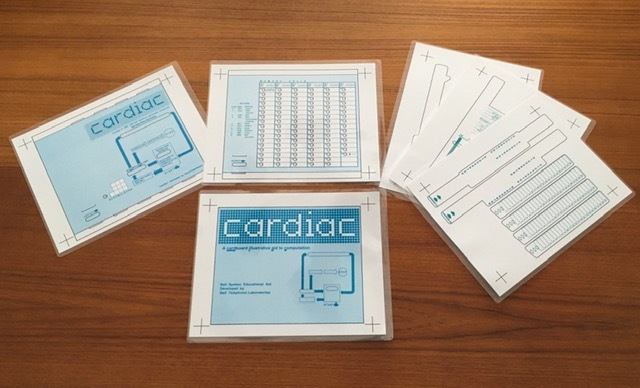
\includegraphics[scale=0.3]{media/CARDIAC_Paper/paper1.jpg}
			\caption{Kit de CARDIAC abierto}
			\label{fig:Kit_CARDIAC}
		\end{figure}
		
		\begin{figure}[h]
			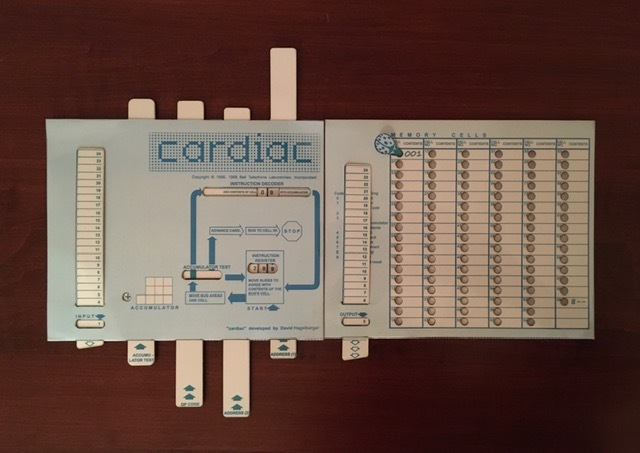
\includegraphics[scale=0.3]{media/CARDIAC_Paper/Construida.jpg}
			\caption{CARDIAC construida}
			\label{fig:CARDIAC_Construida}
		\end{figure}
		
		
		Con esta estructura de papel es posible realizar operaciones básicas que hace una computadora a la vez que puedes ir viendo el proceso que llevan
		los datos desde la entrada(teclado o una tarjeta perforada) hacía la memoria principal y el flujo que sigue la ``maquina'' para ejecutar
		las instrucciones que están en la memoria y diferenciarlas de los datos, así como la interpretación de esas instrucciones, su procesamiento lógico y los
		cáclulos aritmenticos, hasta que llegan al acumulador y de ahí según lo que dicten las instrucciones se puede seguir trabajando con
		esos datos en el acumulador o guardarlos en memoria para su posterior ``impresión'' fuera de la memoria. Este proceso es, muy a grandes rasgos y muy simplificado
		lo que realizan nuestras computadoras hoy en día(con varias mejoras), pero que nosotros no vemos, sólo vemos los resultados, es por está situación que a nosotros
		como estudiantes del siglo 21 que ya contamos con una comptuadora a nuestro alcance, en mayor medida que en los años 60, nos puede ser de útilidad
		CARDIAC para razonar y analizar los procesos que se ejecutan en una comptuadora y entender su funcionamiento; quizá hoy en día un CARDIAC de papel
		no nos sea tan practico, pero el concepto si que lo es, y llevarlo a un entorno electronico que nos de más potencia sin perder la escencia didactica
		de CARDIAC puede ser una gran ayuda para la computación.

		\clearpage		
		
		\subsection{Primeros Sistemas Operativos}
		
		\subsection{Indicios de concurrencia y paralelismo}
	
		\subsection{Actualidad de las computadoras}
		

\chapter{Teoría de la computación} %¿Demasiado pretencioso el titulo?

	\section{Funcionamiento básico de las computadoras}   %% Se podría ampliar a partes más teoricas de automatas
		
		\subsection{Arquitectura Von Neumann}   
	
		\subsection{Sistema Operativo}   	

	\section{Modelos de computo}

		\subsection{Modelo concurrente}

		\subsection{Modelo paralelo}
	
		\subsection{Modelo distribuido}

\chapter{CARDIAC y su evolución}  %
	\section{Operaciones concurrentes}
	
		\subsection{Necesidad de un sistema operativo}
		
		\subsection{Mejoras necesarias en el Hardware}
		
		\subsection{Creación de una arquitectura concurrente}
	
	 \section{Evolución hacia el paralelismo}
	 
	 	\subsection{Hardware y sus necesidades}
	 	
	 	\subsection{Arquitectura paralela E-CARDIAC PAR}


\chapter{Conclusiones}

\newpage

\selectlanguage{spanish}
	\bibliography{CARDIAC}
\selectlanguage{spanish}
	\bibliographystyle{apacite}

%\backmatter%@sglvgdor


\end{document}

